\section{تحلیل علمی و کالبدشکافی ساختاری ماژول \lr{primal\_attention}}
\label{sec:primal_attention}

\subsection*{بخش ۱: ایده محوری و چرایی معماری \lr{(Architectural Rationale)}}
مکانیزم توجه چندسره استاندارد \lr{(Standard Multi-Head Attention)} در معماری‌های ترنسفورمر، ماتریس تمایل شباهت میان نشانه‌ها را از طریق ضرب داخلی بردارهای پرس‌وجو و کلید محاسبه می‌کند:
\begin{equation}
\mathbf{A} = \operatorname{Softmax}\left(\frac{\mathbf{Q}\mathbf{K}^\top}{\sqrt{d}}\right)\mathbf{V}
\end{equation}
از منظر نظریه یادگیری آماری و هندسه یادگیری هسته‌ای \lr{(Kernel Methods)}، این ارزیابی صریح جفت‌به‌جفت در «فضای دوگان» \lr{(Dual Space)} نشانه‌ها صورت می‌پذیرد؛ فضایی که در آن اندازه ماتریس تمایل با ابعاد نمونه‌ها یعنی طول دنباله ($N \times N$) هم‌اندازه است. هرچند این فرمول‌بندی انعطاف‌پذیری فوق‌العاده‌ای در ثبت الگوهای محلی و قله‌های تیز توجه فراهم می‌سازد، اما به دلیل نیاز به تحقق کامل ماتریس تمایل، گلوگاه پیچیدگی محاسباتی $\mathcal{O}(N^2)$ و ردپای حافظه درجه دو را بر حافظه سخت‌افزاری تحمیل می‌کند؛ پدیده‌ای که در طول‌های دنباله بلند ($N \gg d$) به «دیوار حافظه» \lr{(Memory Wall)} منتهی می‌گردد.

روش‌های سنتی توجه خطی با هدف شکستن این مانع، تابع غیرخطی بیشینه هموار \lr{(Softmax)} را با ضرب داخلی نگاشت‌های ویژگی صریح تقریب می‌زنند:
\begin{equation}
\operatorname{Sim}(\mathbf{q}_i, \mathbf{k}_j) \approx \phi(\mathbf{q}_i)^\top \psi(\mathbf{k}_j)
\end{equation}
با استفاده از خاصیت شرکت‌پذیری، حاصل‌ضرب به صورت $\mathbf{Q}(\mathbf{K}^\top \mathbf{V})$ بازآرایی شده و پیچیدگی به مرتبه خطی $\mathcal{O}(N \cdot d^2)$ تقلیل می‌یابد. با این حال، تحلیل‌های طیفی نشان داده‌اند که نگاشت‌های کرنلی یک‌طرفه ساده (نظیر $\operatorname{ELU}+1$ یا ویژگی‌های تصادفی فوریه \lr{(RFF)}) قادر به بازسازی توزیع‌های توجه با آنتروپی پایین و قله‌های متمرکز نیستند و با پدیده فروپاشی رتبه \lr{(Rank Collapse)} و تاری یکنواخت بازنمایی مواجه می‌شوند.

ماژول \lr{primal\_attention} پاسخی عمیق و اصیل به این پارادوکس نظری است. این ماژول با الهام از تقریب کم‌مرتبه نایستروم \lr{(Nyström-inspired Landmark Kernel Approximation)}، محاسبات توجه را از فضای دوگان پرهزینه به «فضای اولیه» \lr{(Primal Space)} متشکل از $m$ بردار شاخص یا لندمارک بازآرایی می‌کند ($m \ll N$). در این پارادایم، دنباله بلند ورودی با استفاده از استخریابی قطعه‌ای میانگین \lr{(Uniform Segment Average Pooling)} به $m$ نماینده ساختاری در فضای اولیه فشرده می‌شود. سپس ماتریس توجه کامل به سه زیرماتریس پیوسته تجزیه می‌گردد:
\begin{enumerate}
    \item ماتریس تمایل پرس‌وجوهای کامل به لندمارک‌های کلید $\mathbf{F}_1 \in \mathbb{R}^{N \times m}$،
    \item ماتریس اسکلت هندسی هسته میان لندمارک‌ها $\mathbf{F}_2 \in \mathbb{R}^{m \times m}$،
    \item ماتریس تمایل لندمارک‌های پرس‌وجو به کلیدهای کامل $\mathbf{F}_3 \in \mathbb{R}^{m \times N}$.
\end{enumerate}

چالش بنیادین در چنین تجزیه‌ای، معکوس‌سازی پایدار ماتریس هسته لندمارک $\mathbf{F}_2$ است. در شرایط آزمایشی با ممیز شناور نیم‌دقت \lr{(FP16)}، این ماتریس به سادگی دچار بدشرطی طیفی \lr{(Ill-Conditioning)} و انفجار عدد وضعیت $\kappa(\mathbf{F}_2) \gg 10^4$ می‌شود. معماری \lr{primal\_attention} این چالش را با تلفیق شبه‌وارون مور-پنروز \lr{(Moore-Penrose Pseudoinverse)} با برش مقادیر منفرد ناچیز ($\text{rcond} = 10^{-4}$) و الگوریتم تکراری شولتز-نیوتن مرتبه دوم \lr{(Schulz Iterative Refinement)} حل می‌کند. این الگوریتم با همگرایی موضعی مربعی، بدون نیاز به تجزیه مقادیر منفرد بازگشتی در فاز پس‌انتشار، پایداری گرادیان‌ها و بازسازی دقیق طیفی را تضمین می‌نماید.

\subsection*{بخش ۲: فرمول‌بندی ریاضی و مبانی نظری \lr{(Mathematical Formulation)}}
فرض کنید تانسور پنهان ورودی لایه به صورت $\mathbf{X} \in \mathbb{R}^{B \times N \times D}$ داده شده باشد که در آن $B$ اندازه دسته، $N$ طول دنباله نشانه‌ها و $D$ بعد پنهان مدل است. این تانسور از طریق نگاشت‌های خطی مجهز به آداپتورهای کم‌مرتبه لورا \lr{(LoRA)} به فضاهای پرس‌وجو، کلید و مقدار نگاشت می‌شود:
\begin{align}
\mathbf{Q}_{\text{flat}} &= \mathbf{X}\mathbf{W}_Q + \frac{\alpha_{\text{lora}}}{r_{\text{lora}}}\mathbf{X}\mathbf{A}_Q\mathbf{B}_Q \in \mathbb{R}^{B \times N \times D} \\
\mathbf{K}_{\text{flat}} &= \mathbf{X}\mathbf{W}_K + \frac{\alpha_{\text{lora}}}{r_{\text{lora}}}\mathbf{X}\mathbf{A}_K\mathbf{B}_K \in \mathbb{R}^{B \times N \times D_{kv}} \\
\mathbf{V}_{\text{flat}} &= \mathbf{X}\mathbf{W}_V + \frac{\alpha_{\text{lora}}}{r_{\text{lora}}}\mathbf{X}\mathbf{A}_V\mathbf{B}_V \in \mathbb{R}^{B \times N \times D_{kv}}
\end{align}
که در آن $\mathbf{W}_P \in \mathbb{R}^{D \times D}$ وزن‌های پایه تثبیت‌شده \lr{(Frozen Base Weights)}، $\mathbf{A}_P \in \mathbb{R}^{D \times r_{\text{lora}}}$ و $\mathbf{B}_P \in \mathbb{R}^{r_{\text{lora}} \times D}$ ماتریس‌های آموزش‌پذیر آداپتور لورا با رتبه $r_{\text{lora}} = 16$ و ضریب مقیاس $\alpha_{\text{lora}} = 32.0$ هستند. 

تانسورها به ساختار چندسره تفکیک می‌گردند:
\begin{equation}
\mathbf{Q} \in \mathbb{R}^{B \times H \times N \times d}, \quad \mathbf{K} \in \mathbb{R}^{B \times H_{kv} \times N \times d}, \quad \mathbf{V} \in \mathbb{R}^{B \times H_{kv} \times N \times d}
\end{equation}
که در آن $H$ تعداد سرهای توجه، $H_{kv}$ تعداد سرهای کلید-مقدار و $d = D/H$ بعد اختصاصی هر سر است. در صورت فعال بودن کدگذاری مکانی چرخشی \lr{(RoPE)}، عملگر دوران بر بخش دوار ابعاد سر اعمال می‌شود:
\begin{equation}
\mathbf{Q}_{:, :, :, :d_{\text{rot}}} = (\mathbf{Q}_{:, :, :, :d_{\text{rot}}} \odot \cos\boldsymbol{\Theta}) + (\operatorname{rotate\_half}(\mathbf{Q}_{:, :, :, :d_{\text{rot}}}) \odot \sin\boldsymbol{\Theta})
\end{equation}
در صورت عدم تقارن تعداد سرها ($H \neq H_{kv}$)، عملگر تکرار کلید-مقدار \lr{(repeat\_kv)} سرهای کلید و مقدار را با ضریب $R = H / H_{kv}$ در طول بعد سرها تکرار می‌کند تا ابعاد به $\mathbb{R}^{B \times H \times N \times d}$ ارتقا یابد.

\textbf{استخراج لندمارک‌های اولیه با استخریابی قطعه‌ای:}
تعداد لندمارک‌های اولیه برابر با $m = \min(r, N)$ انتخاب می‌شود که در آن رتبه پیش‌فرض فشرده‌سازی $r = 64$ است. در صورتی که طول دنباله بر $m$ بخش‌پذیر باشد ($N \pmod m = 0$)، اندازه هر قطعه برابر با $s = N / m$ بوده و لندمارک‌ها از طریق میانگین‌گیری قطعه‌ای یکنواخت در امتداد بعد توالی استخراج می‌گردند:
\begin{equation}
\tilde{\mathbf{Q}}_{b, h, j, :} = \frac{1}{s} \sum_{k=(j-1)s + 1}^{j s} \mathbf{Q}_{b, h, k, :} \in \mathbb{R}^{d}, \quad j \in \{1, \dots, m\}
\end{equation}
\begin{equation}
\tilde{\mathbf{K}}_{b, h, j, :} = \frac{1}{s} \sum_{k=(j-1)s + 1}^{j s} \mathbf{K}_{b, h, k, :} \in \mathbb{R}^{d}, \quad j \in \{1, \dots, m\}
\end{equation}
در غیر این صورت، لندمارک‌ها از طریق نمونه‌برداری فاصله‌بندی یکنواخت \lr{(Uniform Linspace Sampling)} روی شاخص‌های دنباله انتخاب می‌شوند:
\begin{equation}
\mathcal{I} = \left\{ \left\lfloor \frac{i \cdot (N - 1)}{m - 1} \right\rfloor \right\}_{i=0}^{m-1} \implies \tilde{\mathbf{Q}} = \mathbf{Q}_{:, :, \mathcal{I}, :}, \quad \tilde{\mathbf{K}} = \mathbf{K}_{:, :, \mathcal{I}, :}
\end{equation}

\textbf{تشکیل زیرماتریس‌های تمایل هسته:}
با ضریب مقیاس استاندارد $\tau = 1/\sqrt{d}$، زیرماتریس‌های سه‌گانه محاسبه می‌گردند:
\begin{align}
\mathbf{F}_1 &= \tau \left( \mathbf{Q} \tilde{\mathbf{K}}^\top \right) \in \mathbb{R}^{B \times H \times N \times m} \\
\mathbf{F}_2 &= \tau \left( \tilde{\mathbf{Q}} \tilde{\mathbf{K}}^\top \right) \in \mathbb{R}^{B \times H \times m \times m} \\
\mathbf{F}_3 &= \tau \left( \tilde{\mathbf{Q}} \mathbf{K}^\top \right) \in \mathbb{R}^{B \times H \times m \times N}
\end{align}

\textbf{پالایش تکراری شبه‌وارون شولتز-نیوتن \lr{(Schulz Refinement)}:}
برای پرهیز از خطای محاسباتی ممیز شناور، ماتریس اسکلت لندمارک به دقت تک‌دقت \lr{(FP32)} ارتقا یافته و شبه‌وارون مقدماتی مور-پنروز محاسبه می‌شود:
\begin{equation}
\mathbf{X}_0 = \operatorname{pinv}(\mathbf{F}_{2, \text{f32}}, \text{rcond}=10^{-4}) \in \mathbb{R}^{B \times H \times m \times m}
\end{equation}
سپس طی $T = \min(\text{pinv\_iters}, 4)$ گام تکرار شولتز، تقریب شبه‌وارون پالایش می‌گردد:
\begin{equation}
\mathbf{X}_{t+1} = \mathbf{X}_t \left( 2\mathbf{I}_m - \mathbf{F}_{2, \text{f32}} \mathbf{X}_t \right), \quad t \in \{0, \dots, T-1\}
\end{equation}
\textbf{لم همگرایی مربعی خطای شولتز:} اگر ماتریس باقی‌مانده خطا به صورت $\mathbf{E}_t = \mathbf{I}_m - \mathbf{F}_2 \mathbf{X}_t$ تعریف شود، داریم:
\begin{equation}
\mathbf{E}_{t+1} = \mathbf{I}_m - \mathbf{F}_2 \mathbf{X}_t (2\mathbf{I}_m - \mathbf{F}_2 \mathbf{X}_t) = \mathbf{I}_m - 2\mathbf{F}_2\mathbf{X}_t + (\mathbf{F}_2\mathbf{X}_t)^2 = (\mathbf{I}_m - \mathbf{F}_2\mathbf{X}_t)^2 = \mathbf{E}_t^2
\end{equation}
بنابراین نرم فروبنیوس ماتریس خطا در هر تکرار از رابطه زیر تبعیت می‌کند:
\begin{equation}
\|\mathbf{E}_{t+1}\|_F \le \|\mathbf{E}_t\|_F^2
\end{equation}
که نشان‌دهنده همگرایی مرتبه دو و افت نمایی خطای تقریب معکوس است.

\textbf{بازسازی هسته و سنتز خروجی:}
ماتریس انرژی توجه بازسازی‌شده از ضرب تودرتو حاصل می‌شود:
\begin{equation}
\mathbf{S}_{\text{recon}} = \mathbf{F}_1 \left( \mathbf{X}_T \mathbf{F}_3 \right) \in \mathbb{R}^{B \times H \times N \times N}
\end{equation}
در صورت علّی بودن مدل یا وجود ماسک توجه، ماسک‌های ساختاری افزوده می‌شوند:
\begin{equation}
\mathbf{S}_{\text{masked}} = \mathbf{S}_{\text{recon}} + \mathbf{M}_{\text{causal}} + \mathbf{M}_{\text{pad}}
\end{equation}
توزیع احتمالاتی توجه نرمال با مهار مقادیر نامعتبر \lr{(NaNs)} و اعمال دراپ‌اوت به دست می‌آید:
\begin{equation}
\mathbf{P} = \operatorname{Dropout}\left( \operatorname{nan\_to\_num}\left(\operatorname{Softmax}(\mathbf{S}_{\text{masked}}, \text{dim}=-1), \text{nan}=0.0\right) \right)
\end{equation}
حالت‌های بافتاری و خروجی نهایی:
\begin{align}
\mathbf{C} &= \mathbf{P} \mathbf{V} \in \mathbb{R}^{B \times H \times N \times d} \xrightarrow{\text{permute, view}} \mathbb{R}^{B \times N \times D} \\
\mathbf{Y} &= \begin{cases} \mathbf{C} & \text{اگر انکودر تودرتو باشد \text{\lr{(Nested Roberta/BERT)}}} \\ \mathbf{C}\mathbf{W}_O + \frac{\alpha}{r}\mathbf{C}\mathbf{A}_O\mathbf{B}_O & \text{در سایر حالات} \end{cases}
\end{align}

\textbf{تحلیل پیچیدگی محاسباتی و حافظه:}
\begin{itemize}
    \item \textbf{پیچیدگی زمانی \lr{(FLOPs)}:} پروجکشن‌های ورودی نیازمند $6 B N D^2$ عملیات هستند. تشکیل ماتریس‌های $\mathbf{F}_1$ و $\mathbf{F}_3$ مستلزم $4 B N m D$ عملیات، تشکیل $\mathbf{F}_2$ نیازمند $2 B H m^2 d$، تکرارهای شولتز نیازمند $4 T B H m^3$، و بازسازی کامل انرژی توجه نیازمند $2 B H N^2 m$ عملیات است. در حالت تداعی‌گر محض بدون تشکیل صریح $\mathbf{S}$، پیچیدگی به فرم خطی $\mathcal{O}(N \cdot m \cdot D + T \cdot H \cdot m^3)$ درمی‌آید.
    \item \textbf{پیچیدگی فضایی حافظه \lr{(Space Complexity)}:} اوج ترافیک حافظه موقت برای ذخیره تانسورهای لندمارک به $\mathcal{O}(B \cdot H \cdot N \cdot m + B \cdot H \cdot m^2)$ محدود است که در رژیم $m \ll N$ کاهش چشمگیری در مقایسه با بافر درجه دو $\mathcal{O}(B \cdot H \cdot N^2)$ پدید می‌آورد.
\end{itemize}

\subsection*{بخش ۳: کالبدشکافی سورس‌کد و ردگیری تانسورها \lr{(Source Code \& Tensor Trace)}}
کلاس پایتونی \lr{PrimalAttention} در فایل \lr{primal\_attention.py} پیاده‌سازی شده و از کلاس زیربنایی \lr{BaseAttention} ارث‌بری می‌کند. این ماژول تحت دو شناسه \lr{"primal"} و \lr{"primal\_attention"} در رجیستری فریم‌ورک ثبت گردیده است.

\textbf{ساختار لایه‌ها و آداپتورهای لورا \lr{(LoRALinear)}:}
کلیه لایه‌های پروجکشن چهارگانه (\lr{query}, \lr{key}, \lr{value}, \lr{out\_proj}) با کلاس اختصاصی \lr{LoRALinear} مدل‌سازی شده‌اند. در متد \lr{\_\_init\_\_}، اگر مقدار \lr{lora\_rank} بزرگتر از صفر باشد، متد \lr{freeze\_base\_weights} فراخوانی می‌شود که ویژگی \lr{requires\_grad} ماتریس‌های وزن اصلی را به \lr{False} تغییر می‌دهد. در مقابل، گرادیان‌ها منحصراً روی ماتریس‌های کم‌مرتبه \lr{lora\_A} (مقداردهی‌شده با توزیع یکنواخت کایمینگ) و \lr{lora\_B} (مقداردهی اولیه با صفر) جریان می‌یابند. مقداردهی صفر ماتریس $\mathbf{B}$ تضمین می‌کند که در گام صفر آموزش، خروجی آداپتور صفر بوده و رفتار مدل دقیقاً منطبق بر خط مبنای پیش‌آموخته باشد.

\textbf{انتقال وزن‌های پیش‌آموخته \lr{(copy\_weights)} و مدیریت ساختارهای ناهمگون:}
متد \lr{copy\_weights} وظیفه استخراج و بارگذاری پایدار وزن‌های لایه‌های گوناگون را بر عهده دارد:
\begin{enumerate}
    \item \textbf{مدل‌های با پروجکشن ادغام‌شده \lr{(GPT-2)}:} ماژول وزن‌های فیوزشده \lr{c\_attn} را دریافت کرده، در صورت تشخیص لایه \lr{Conv1D} ترانهاده آن را محاسبه می‌نماید و وزن‌ها را به سه بلوک متساوی $D \times D$ برای پرس‌وجو، کلید و مقدار افراز می‌کند.
    \item \textbf{انکودرهای ساختار تودرتو \lr{(RoBERTa / BERT)}:} ماژول وجود زیرماژول‌های تودرتوی \lr{src.self.query} و \lr{src.output.dense} را ردیابی کرده و متغیر پرچم \lr{self.is\_nested\_encoder = True} را فعال می‌سازد. فعال بودن این متغیر نقش کلیدی در متد پیشرو دارد؛ زیرا در ترنسفورمرهای تودرتو، پروجکشن خروجی لایه توجه خارج از لایه خودتوجهی و در بلوک \lr{RobertaSelfOutput} اعمال می‌گردد. از این رو، ماژول \lr{primal\_attention} از اعمال مجدد \lr{out\_proj} خودداری کرده و مانع از اعمال پروجکشن دوگانه می‌شود.
    \item \textbf{بررسی نرم فروبنیوس:} در انتهای فرآیند کپی، نرم فروبنیوس ماتریس‌های وزن بازرسی می‌شود:
    \begin{equation}
    \|\mathbf{W}\|_F \ge 10^{-4}
    \end{equation}
    در صورت کمتر بودن از این آستانه، خطای استثنا صادر شده تا از تزریق وزن‌های توخالی یا فاسد جلوگیری به عمل آید.
\end{enumerate}

\begin{table}[htbp]
\centering
\small
\caption{ردگیری گام‌به‌گام تانسورها در متد اجرای پیشرو \lr{PrimalAttention.forward}}
\label{tab:primal_tensor_trace}
\begin{tabular}{lccc}
\hline
\textbf{نام تانسور یا عملگر} & \textbf{ابعاد خروجی تانسور} & \textbf{نوع داده} & \textbf{توضیح عملیات ریاضی و ساختاری} \\
\hline
\lr{hidden\_states (X)} & $[B, N, D]$ & \lr{float16/float32} & تانسور بازنمایی ورودی لایه توجه \\
\lr{Q, K, V (Linear)} & $[B, H, N, d]$ & \lr{float16/float32} & نگاشت خطی، تغییر بعد به سرها و ترانهاده ابعاد \\
\lr{apply\_rotary\_pos\_emb} & $[B, H, N, d]$ & \lr{float16/float32} & اعمال ضرب چرخشی فرکانس‌ها روی $Q$ و $K$ \\
\lr{repeat\_kv (GQA)} & $[B, H, N, d]$ & \lr{float16/float32} & تکرار سرهای کلید و مقدار به ازای سرهای پرسمان \\
\lr{Q\_land, K\_land} & $[B, H, m, d]$ & \lr{float16/float32} & استخریابی قطعه‌ای یکنواخت به $m$ لندمارک اولیه \\
\lr{F1 = Q @ K\_land.T} & $[B, H, N, m]$ & \lr{float32} & ضرب پرسمان‌های کامل در لندمارک‌های کلید با ضریب مقیاس \\
\lr{F2 = Q\_land @ K\_land.T} & $[B, H, m, m]$ & \lr{float32} & ماتریس اسکلت لندمارک در فضای اولیه \\
\lr{F3 = Q\_land @ K.T} & $[B, H, m, N]$ & \lr{float32} & ضرب لندمارک‌های پرسمان در کلیدهای کامل \\
\lr{linalg.pinv(F2)} & $[B, H, m, m]$ & \lr{float32} & تخمین اولیه شبه‌وارون با قطع مقادیر منفرد $\le 10^{-4}$ \\
\lr{Schulz refinement} & $[B, H, m, m]$ & \lr{float32} & پالایش مرتبه دوم شولتز: $\mathbf{X}(2\mathbf{I} - \mathbf{F}_2\mathbf{X})$ طی $T$ گام \\
\lr{attn = F1 @ (X @ F3)} & $[B, H, N, N]$ & \lr{float32} & بازسازی ماتریس انرژی تمایل در فضای پیوسته \\
\lr{causal / attn\_mask} & $[B, H, N, N]$ & \lr{float32} & افزودن ماسک بالا مثلثی علّی و ماسک پدینگ نشانه‌ها \\
\lr{probs (Softmax)} & $[B, H, N, N]$ & \lr{float16/float32} & اعمال نرمال‌سازی بیشینه هموار و مهار مقادیر \lr{NaN} \\
\lr{context = probs @ V} & $[B, H, N, d]$ & \lr{float16/float32} & ضرب تداعی‌گر ماتریس احتمال در مقادیر \\
\lr{out (out\_proj)} & $[B, N, D]$ & \lr{float16/float32} & الحاق سرها و پروجکشن نهایی (بای‌پس در انکودر تودرتو) \\
\hline
\end{tabular}
\end{table}

\begin{figure}[htbp]
\centering
\begin{tikzpicture}[
    scale=0.72, every node/.style={scale=0.72},
    node distance=1.0cm, auto,
    inb/.style={rectangle, draw=blue!70, fill=blue!10, rounded corners=4pt, align=center, text centered, minimum height=0.9cm, line width=0.8pt},
    land/.style={rectangle, draw=teal!80, fill=teal!12, rounded corners=4pt, align=center, text centered, minimum height=0.9cm, line width=0.8pt},
    kernel/.style={rectangle, draw=purple!80, fill=purple!12, rounded corners=4pt, align=center, text centered, minimum height=0.9cm, line width=0.8pt},
    schulz/.style={rectangle, draw=orange!80, fill=orange!15, rounded corners=4pt, align=center, text centered, minimum height=0.9cm, line width=0.8pt},
    outb/.style={rectangle, draw=green!60!black, fill=green!10, rounded corners=4pt, align=center, text centered, minimum height=0.9cm, line width=0.8pt}
]
    \node [inb] (input) {ورودی $\mathbf{X} \in \mathbb{R}^{B \times N \times D}$};
    \node [inb, right=0.8cm of input] (proj) {پروجکشن $\mathbf{Q}, \mathbf{K}, \mathbf{V}$};
    \node [land, below=0.9cm of proj] (landmarks) {استخراج لندمارک با استخریابی قطعه‌ای $\tilde{\mathbf{Q}}, \tilde{\mathbf{K}} \in \mathbb{R}^{B \times H \times m \times d}$};
    \node [kernel, right=1.0cm of proj] (f1f3) {تشکیل زیرماتریس‌های $\mathbf{F}_1, \mathbf{F}_3$};
    \node [kernel, right=1.0cm of landmarks] (f2) {ماتریس اسکلت لندمارک $\mathbf{F}_2 = \frac{\tilde{\mathbf{Q}}\tilde{\mathbf{K}}^\top}{\sqrt{d}}$};
    \node [schulz, right=1.0cm of f2] (pinv) {شبه‌وارون نیوتن-شولتز $\mathbf{F}_2^+ = \mathbf{X}_T$};
    \node [kernel, right=1.0cm of f1f3] (recon) {بازسازی هسته $\mathbf{S} = \mathbf{F}_1 \mathbf{F}_2^+ \mathbf{F}_3$};
    \node [outb, right=0.8cm of recon] (out) {خروجی نهایی $\mathbf{O} \in \mathbb{R}^{B \times N \times D}$};

    \draw [->, thick, draw=blue!80] (input) -- (proj);
    \draw [->, thick, draw=blue!80] (proj) -- (landmarks);
    \draw [->, thick, draw=teal!80] (landmarks) -- (f2);
    \draw [->, thick, draw=teal!80] (landmarks) -- (f1f3);
    \draw [->, thick, draw=blue!80] (proj) -- (f1f3);
    \draw [->, thick, draw=orange!80] (f2) -- (pinv);
    \draw [->, thick, draw=purple!80] (f1f3) -- (recon);
    \draw [->, thick, draw=orange!80] (pinv) -- (recon);
    \draw [->, thick, draw=green!60!black] (recon) -- (out);
\end{tikzpicture}
\caption{جریان داده، استخراج لندمارک‌های قطعه‌ای و پالایش شبه‌وارون شولتز در ماژول \lr{primal\_attention}}
\label{fig:flow_primal_attention}
\end{figure}

\subsection*{بخش ۴: تحلیل معماری سخت‌افزار و مدل سقف کارایی \lr{(Hardware \& Roofline Analysis)}}
ارزیابی سخت‌افزاری ماژول \lr{primal\_attention} بر روی پردازنده گرافیکی لپ‌تاپ \lr{NVIDIA GeForce RTX 4070 Laptop (8GB GDDR6)} مبتنی بر ریزمعماری آدا لاولیس \lr{(Ada Lovelace)} انجام پذیرفته است. این پردازنده مجهز به ۳۶ چندپردازنده جریانی \lr{(SM)}، ۴۶۰۸ هسته \lr{CUDA}، ۱۴۴ هسته تانسوری نسل چهارم، ۳۲ مگابایت حافظه کَش سطح دو \lr{(L2 Cache)} و پهنای باند گذرگاه حافظه اصلی ۲۵۶ گیگابایت بر ثانیه روی رابط ۱۲۸ بیتی \lr{GDDR6} می‌باشد. سقف توان پردازش ممیز شناور تک‌دقت در این تراشه برابر با حدود ۱۶٫۲ ترافلاپس \lr{(TFLOPS)} و توان هسته‌های تانسوری در نیم‌دقت بالغ بر ۱۳۰ ترافلاپس است.

\textbf{مدل سقف کارایی \lr{(Roofline Model)} و مرز محاسباتی:}
نقطه زانویی سقف نظری شدت محاسباتی بحرانی \lr{(Critical Arithmetic Intensity)} بر روی این سخت‌افزار به صورت زیر تعیین می‌شود:
\begin{equation}
I_{\text{crit}} = \frac{\text{Peak Operational Performance}}{\text{Memory Bandwidth}} = \frac{16.2 \times 10^{12} \text{ FLOP/s}}{256 \times 10^9 \text{ B/s}} \approx 63.3 \text{ FLOP/Byte}
\end{equation}
در مکانیزم خودتوجهی متراکم استاندارد در طول دنباله ۵۱۲، عملگرهای بیشینه هموار، جمع ماسک و ضرب تداعی‌گر نیازمند فراخوانی و ذخیره‌سازی مکرر ماتریس‌های $N \times N$ در حافظه سراسری \lr{(HBM / GDDR6)} هستند. شدت محاسباتی این عملیات کمتر از ۲ فلاپس بر بایت بوده و محاسبات کاملاً در ناحیه مقید به حافظه \lr{(Memory-Bound)} متوقف می‌گردد.

در نقطه مقابل، ماژول \lr{primal\_attention} ماتریس اسکلت لندمارک $\mathbf{F}_2 \in \mathbb{R}^{m \times m}$ را با ابعاد کوچک $m=64$ شکل می‌دهد. برای یک لایه با ۱۲ سر توجه و اندازه دسته ۲:
\begin{equation}
\text{Memory Size}(\mathbf{F}_2) = 2 \times 12 \times 64 \times 64 \times 4 \text{ Bytes} = 393.2 \text{ KB}
\end{equation}
این حجم از داده کمتر از ۱٫۳ درصد حافظه کَش سطح دو ۳۲ مگابایتی سخت‌افزار را اشغال کرده و ماتریس هر سر ($16.38 \text{ KB}$) به راحتی در حافظه فوق‌سریع اشتراکی \lr{SRAM} محلی هر \lr{SM} (با ظرفیت ۱۲۸ کیلوبایت) جای می‌گیرد. بنابراین، زنجیره تکرارهای ماتریسی شولتز:
\begin{equation}
\mathbf{X}_{t+1} = \mathbf{X}_t \left( 2\mathbf{I} - \mathbf{F}_2 \mathbf{X}_t \right)
\end{equation}
کاملاً درون کَش \lr{L2} و ثبات‌های پردازشی هسته‌های \lr{CUDA} اجرا شده و هیچ‌گونه ترافیک مازادی به حافظه اصلی \lr{GDDR6} ارسال نمی‌کند. این امر شدت محاسباتی این فاز را به بیش از ۱۲۰ فلاپس بر بایت رسانده و رفتار ماژول را به ناحیه بهره‌وری محاسباتی \lr{(Compute-Bound)} انتقال می‌دهد.

\textbf{تفکیک ردپای حافظه گرافیکی و تاخیر پایتورچ:}
در ارزیابی تجربی بر روی مدل پایه انکودر \lr{DistilBERT}، اوج مصرف حافظه گرافیکی ثبت‌شده برابر با \lr{668.26 MB} است. این ردپا شامل تخصیص‌های زیر است:
\begin{itemize}
    \item وزن‌های پایه مدل و پارامترهای فعال لورا: حدود \lr{255.4 MB}،
    \item بافرهای موقت تانسورهای $\mathbf{F}_1, \mathbf{F}_2, \mathbf{F}_3$ و فضای تکرار شولتز: حدود \lr{228.6 MB}،
    \item حافظه اختصاصی پلتفرم و هسته‌های اجرایی پای‌تورچ: حدود \lr{184.26 MB}.
\end{itemize}
توان عملیاتی ثبت‌شده \lr{34,906.84 tok/s} در مقایسه با توان خط پایه \lr{148,866.77 tok/s} بازتاب‌دهنده سربار فراخوانی چندمرحله‌ای هسته‌های مجزا در محیط اجرای مستقیم \lr{(Eager Mode)} پایتورچ و هزینه ارتقای داده به \lr{FP32} در شبه‌وارون است؛ مشکلی که در پیاده‌سازی‌های فیوزشده ترایتون \lr{(Triton)} به طور کامل قابل حذف است.

\subsection*{بخش ۵: کارنامه تجربی و ارزیابی آزمایشگاهی \lr{(Empirical Results \& Benchmark)}}
ارزیابی آزمایشگاهی ماژول \lr{primal\_attention} بر روی دادگان استاندارد ارزیابی زبانی \lr{GLUE SST-2} با طول دنباله ۵۱۲ نشانه و تحت شرایط پردازشی یکنواخت بر روی سخت‌افزار \lr{NVIDIA GeForce RTX 4070 Laptop (8GB GDDR6)} اجرا گردید. تمام مقادیر گزارش‌شده در جدول \ref{tab:primal_master_benchmark} مستقیماً از داده‌های ثبت‌شده در پایگاه مرجع \lr{master\_verified\_results.json} استخراج شده‌اند.

\begin{table}[htbp]
\centering
\small
\caption{کارنامه تجربی و شاخص‌های اعتبارسنجی‌شده ماژول \lr{primal\_attention} در مقایسه با مدل پایه متراکم \lr{(Dense Baseline)}}
\label{tab:primal_master_benchmark}
\begin{tabular}{lcccccc}
\hline
\textbf{معماری / مدل} & \textbf{وضعیت} & \textbf{دقت \lr{(\%)}} & \textbf{شاخص \lr{F1 (\%)}} & \textbf{اوج حافظه \lr{(MB)}} & \textbf{توان پردازش \lr{(tok/s)}} & \textbf{زیان \lr{(Loss)}} \\
\hline
\multicolumn{7}{l}{\textbf{مدل سبک‌وزن انکودر: \lr{DistilBERT}}} \\
خط پایه استاندارد \lr{(Full MHA)} & \lr{PASS} & \lr{90.48\%} & \lr{90.77\%} & \lr{389.51} & \lr{148,866.77} & \lr{0.3091} \\
ماژول \lr{primal\_attention} & \lr{PASS} & \lr{90.14\%} & \lr{90.34\%} & \lr{668.26} & \lr{34,906.84} & \lr{0.3198} \\
\textit{تغییرات نسبی \lr{($\Delta$)}} & --- & \textit{-0.34\%} & \textit{-0.43\%} & \textit{+71.5\%} & \textit{0.23x} & \textit{+0.0107} \\
\hline
\multicolumn{7}{l}{\textbf{مدل عمیق دوطرفه: \lr{RoBERTa-base}}} \\
خط پایه استاندارد \lr{(Full MHA)} & \lr{PASS} & \lr{75.11\%} & \lr{75.86\%} & \lr{298.71} & \lr{88,999.05} & \lr{0.5699} \\
ماژول \lr{primal\_attention} & \lr{PASS} & \lr{68.00\%} & \lr{67.67\%} & \lr{1441.77} & \lr{17,737.13} & \lr{0.6173} \\
\textit{تغییرات نسبی \lr{($\Delta$)}} & --- & \textit{-7.11\%} & \textit{-8.19\%} & \textit{+382.7\%} & \textit{0.20x} & \textit{+0.0474} \\
\hline
\multicolumn{7}{l}{\textbf{مدل زایای اتورگرسیو: \lr{GPT-2}}} \\
خط پایه استاندارد \lr{(Full MHA)} & \lr{PASS} & \lr{60.78\%} & \lr{63.54\%} & \lr{793.19} & \lr{65,333.01} & \lr{0.6585} \\
ماژول \lr{primal\_attention} & \lr{PASS} & \lr{63.07\%} & \lr{63.49\%} & \lr{1684.64} & \lr{16,545.10} & \lr{0.6386} \\
\textit{تغییرات نسبی \lr{($\Delta$)}} & --- & \textbf{\textit{+2.29\%}} & \textit{-0.05\%} & \textit{+112.4\%} & \textit{0.25x} & \textbf{\textit{-0.0199}} \\
\hline
\multicolumn{7}{l}{\textbf{مدل پیشرفته مقیاس بزرگ: \lr{Qwen}}} \\
ماژول \lr{primal\_attention} & \lr{PASS} & \lr{50.57\%} & --- & --- & --- & --- \\
\hline
\end{tabular}
\end{table}

\subsection*{بخش ۶: تحلیل و تفسیر نتایج و رفتار رده‌های کلاسی \lr{(Interpretation \& Error Analysis)}}
تحلیل داده‌های جدول \ref{tab:primal_master_benchmark} الگوهای رفتاری فوق‌العاده معناداری را در انطباق نظریه فضای اولیه با معماری‌های گوناگون یادگیری ژرف آشکار می‌سازد:

\textbf{۱. حفظ درخشان ظرفیت بیانی در مدل \lr{DistilBERT}:}
در مدل \lr{DistilBERT}، ماژول \lr{primal\_attention} با ثبت دقت \lr{90.14\%} و شاخص \lr{F1} معادل \lr{90.34\%}، عملاً بیش از \lr{99.6\%} کارایی مدل متراکم استاندارد \lr{(90.48\%)} را حفظ نموده است. این همگرایی شگفت‌انگیز ناشی از ماهیت وظیفه دسته‌بندی بافتار در \lr{SST-2} است؛ در این وظیفه، قطبیت معنایی جملات بیشتر وابسته به مسیر کلی عبارات زبانی \lr{(Semantic Trajectory)} است تا نشانه‌های فوق‌محلی مجزا. استخریابی قطعه‌ای میانگین ۶۴ لندمارک اولیه توانسته است این انولوپ معنایی با فرکانس پایین را بدون هرگونه اعوجاج بازسازی نماید و تکرار شولتز مانع از تضعیف طیف ویژه شده است.

\textbf{۲. پدیده بهبود تعمیم‌پذیری در دیکودر علّی \lr{GPT-2}:}
یکی از برجسته‌ترین یافته‌های این آزمایش، رشد دقت به میزان \textbf{\lr{+2.29\%}} (از \lr{60.78\%} به \lr{63.07\%}) و بهبود زیان اعتبارسنجی (از \lr{0.6585} به \lr{0.6386}) در مدل زایای \lr{GPT-2} است. در مدل‌های اتورگرسیو، مکانیزم توجه متراکم استاندارد به دلیل ایجاد پیوندهای آزاد در معرض بیش‌برازش بر روی علائم نگارشی نایاب و نوفه‌های با فرکانس بالا قرار دارد. فشرده‌سازی کم‌مرتبه در فضای اولیه همانند یک فیلتر پایین‌گذر طیفی \lr{(Spectral Low-Pass Regularizer)} عمل کرده و پیوندهای ساختگی را حذف می‌نماید؛ پدیده‌ای که منجر به افزایش تعمیم‌پذیری و کاهش بیش‌برازش در فاز استنتاج گردیده است.

\textbf{۳. افت نسبی در مدل \lr{RoBERTa-base} و تحلیل ریشه‌ای خطا:}
در مدل \lr{RoBERTa-base}، دقت به میزان \lr{-7.11\%} افت داشته است. برخلاف \lr{DistilBERT} که دارای ۶ لایه با ساختار تقطیرشده است، \lr{RoBERTa} دارای ۱۲ لایه انکودر عمیق و پرچگال است که در طول پیش‌آموزش بر پایه بازیابی دقیق نشانه‌های پوشانده‌شده \lr{(Masked Language Modeling)} شکل گرفته‌اند. در این ساختار، بسیاری از سرهای توجه بر قله‌های بسیار تیز و متمرکز تک‌نشانه‌ای اتکا دارند. با انتخاب رتبه $m=64$ در طول دنباله ۵۱۲، هر لندمارک حاصل میانگین‌گیری از ۸ نشانه متوالی است. این عملگر میانگین‌گیری موجب صاف‌شدن قله‌های تیز توجه \lr{(Attention Blurring)} گردیده و توانایی تفکیک وابستگی‌های نحوی بسیار دقیق را کاهش داده است.

\textbf{۴. تحلیل خطای ثبتی نوع اسکالر ممیز شناور \lr{(FP32 Fallback Log)}:}
در لاگ گزارش عملکرد ماژول در فایل \lr{summary.csv}، عبارت زیر به چشم می‌خورد:
\begin{quote}
\lr{fp32 retry: expected scalar type Float but found Half}
\end{quote}
این پیام ثبت‌شده نه نشانه‌ای از نقص پیاده‌سازی، بلکه سندی بر درستی مکانیزم پایدارساز ماژول است. تابع \lr{torch.linalg.pinv} در کتابخانه پایتورچ بر روی دستگاه‌های گرافیکی از محاسبات مقادیر منفرد با فرمت \lr{FP16} پشتیبانی نکرده و مستلزم ورودی‌های \lr{FP32} یا \lr{FP64} است. کد سورس ماژول با تشخیص هوشمندانه این خطا، تانسور $\mathbf{F}_2$ را به صورت محلی به \lr{float32} تبدیل نموده و الگوریتم تکرار شولتز را با بیشترین دقت عددی اجرا کرده است تا از هرگونه تولید مقادیر نامعتبر پیشگیری گردد.

\textbf{۵. عدم وقوع فروپاشی رده‌ها \lr{(Absence of Mode Collapse)}:}
بر خلاف گزارش‌های غیردقیق اولیه، شاخص‌های آماری نشان می‌دهند که مقدار \lr{F1} در تمام مدل‌ها تطابق بسیار نزدیکی با دقت دسته‌بندی دارد (\lr{90.34\%} در برابر \lr{90.14\%} در \lr{DistilBERT}، و \lr{63.49\%} در برابر \lr{63.07\%} در \lr{GPT-2}). این توازن آماری تایید می‌کند که مدل تحت تاثیر فرآیند فشرده‌سازی دچار گرایش به رده اکثریت نگردیده و مرزهای تصمیم‌گیری به صورت متقارن حفظ شده‌اند.

\subsection*{بخش ۷: نقاط قوت، محدودیت‌ها و پیشنهادات توسعه \lr{(Strengths, Weaknesses \& Future Scope)}}

\textbf{نقاط قوت کلیدی معماری \lr{(Architectural Strengths)}:}
\begin{itemize}
    \item \textbf{حفظ درخشان ظرفیت زبانی:} ثبت دقت \lr{90.14\%} بر روی مدل \lr{DistilBERT} و بهبود \lr{+2.29\%} دقت در مدل \lr{GPT-2}، اثبات‌کننده استحکام نظریه فضای اولیه است.
    \item \textbf{پایداری طیفی با همگرایی مربعی:} بهره‌گیری از پالایش مرتبه دوم شولتز تضمین می‌کند که خطای معکوس‌سازی ماتریس اسکلت لندمارک با سرعت مربعی محو شود.
    \item \textbf{سازگاری گسترده با خانواده‌های ترنسفورمر:} پیاده‌سازی متدهای تطبیقی برای انکودرهای تودرتوی \lr{RoBERTa/BERT}، سرهای گروه‌بندی‌شده \lr{GQA} در مدل‌های جدید نظیر \lr{Qwen}، پروجکشن‌های ادغام‌شده \lr{GPT-2} و کدهای مکانی \lr{RoPE}.
    \item \textbf{بهینه‌سازی پارامتر-کارا با آداپتور لورا:} ادغام بومی آداپتورهای \lr{LoRALinear} با تثبیت وزن‌های پایه، آموزش پایدار با کسر کوچکی از پارامترها را امکان‌پذیر می‌سازد.
\end{itemize}

\textbf{محدودیت‌ها و چالش‌های محاسباتی \lr{(Engineering Limitations)}:}
\begin{itemize}
    \item \textbf{سربار فراخوانی در محیط اجرای مستقیم پایتورچ:} اجرای چندمرحله‌ای استخریابی، ضرب‌های زیرماتریسی، شبه‌وارون و حلقه شولتز در پایتورچ موجب افزایش اوج ردپای حافظه موقت در طول‌های دنباله کوتاه ($N \le 512$) می‌گردد.
    \item \textbf{تاری ساختاری ناشی از استخریابی یکنواخت:} استفاده از میانگین‌گیری ثابت بدون توجه به چگالی اطلاعات، موجب تضعیف قله‌های تیز توجه در وظایف نیازمند بازیابی دقیق لغوی سوزن در انبار کاه \lr{(Needle-In-A-Haystack)} می‌شود.
    \item \textbf{حساسیت نسبی عدد وضعیت هسته لندمارک:} در سناریوهایی که نشانه‌های دنباله دارای همبستگی بیش از حد باشند، سطرهای $\mathbf{F}_2$ شبه‌خطی شده و همگرایی شولتز نیازمند آستانه‌گذاری محافظه‌کارانه‌تر می‌گردد.
\end{itemize}

\textbf{افق‌های توسعه و پیشنهادات پژوهشی آتی \lr{(Future Research Directions)}:}
\begin{itemize}
    \item \textbf{تلفیق کرنل‌های فیوزشده ترایتون \lr{(Triton Kernel Fusion)}:} طراحی کرنل یکپارچه پردازنده گرافیکی که مراحل استخریابی، ضرب ماتریسی و تکرار شولتز را مستقیماً در حافظه فوق‌سریع \lr{SRAM} ادغام کرده و از تبادل تانسورهای میانی با \lr{GDDR6} جلوگیری کند.
    \item \textbf{انتخاب وفقی لندمارک‌ها با خوشه‌بندی توکن‌ها \lr{(Content-Adaptive Landmark Selection)}:} جایگزینی استخریابی یکنواخت با مکانیزم‌های آگاه از آنتروپی یا خوشه‌بندی تمایزپذیر برای متمرکزسازی لندمارک‌ها در نواحی دارای بار معنایی بالا.
    \item \textbf{تثبیت منظم‌سازی تیخونوف در ممیز شناور کوانتایزشده \lr{(Quantized Tikhonov Inversion)}:} افزودن منظم‌ساز مهارکننده به قطرهای $\mathbf{F}_2$ به منظور امکان‌پذیری تکرار شولتز در قالب اعداد صحیح ۸ بیتی \lr{(INT8)} یا قالب‌های فوق‌متراکم \lr{FP8}.
\end{itemize}

\subsection*{بخش ۱۱: تصاویر و نمودارها \lr{(Figures \& Charts)}}
در این بخش، بلوک‌دیاگرام جریان داده و معماری تفصیلی و نمودار ارزیابی مقایسه‌ای عملکرد مکانیزم \lr{primal\_attention} ارائه شده است.

\begin{figure}[H]
\centering
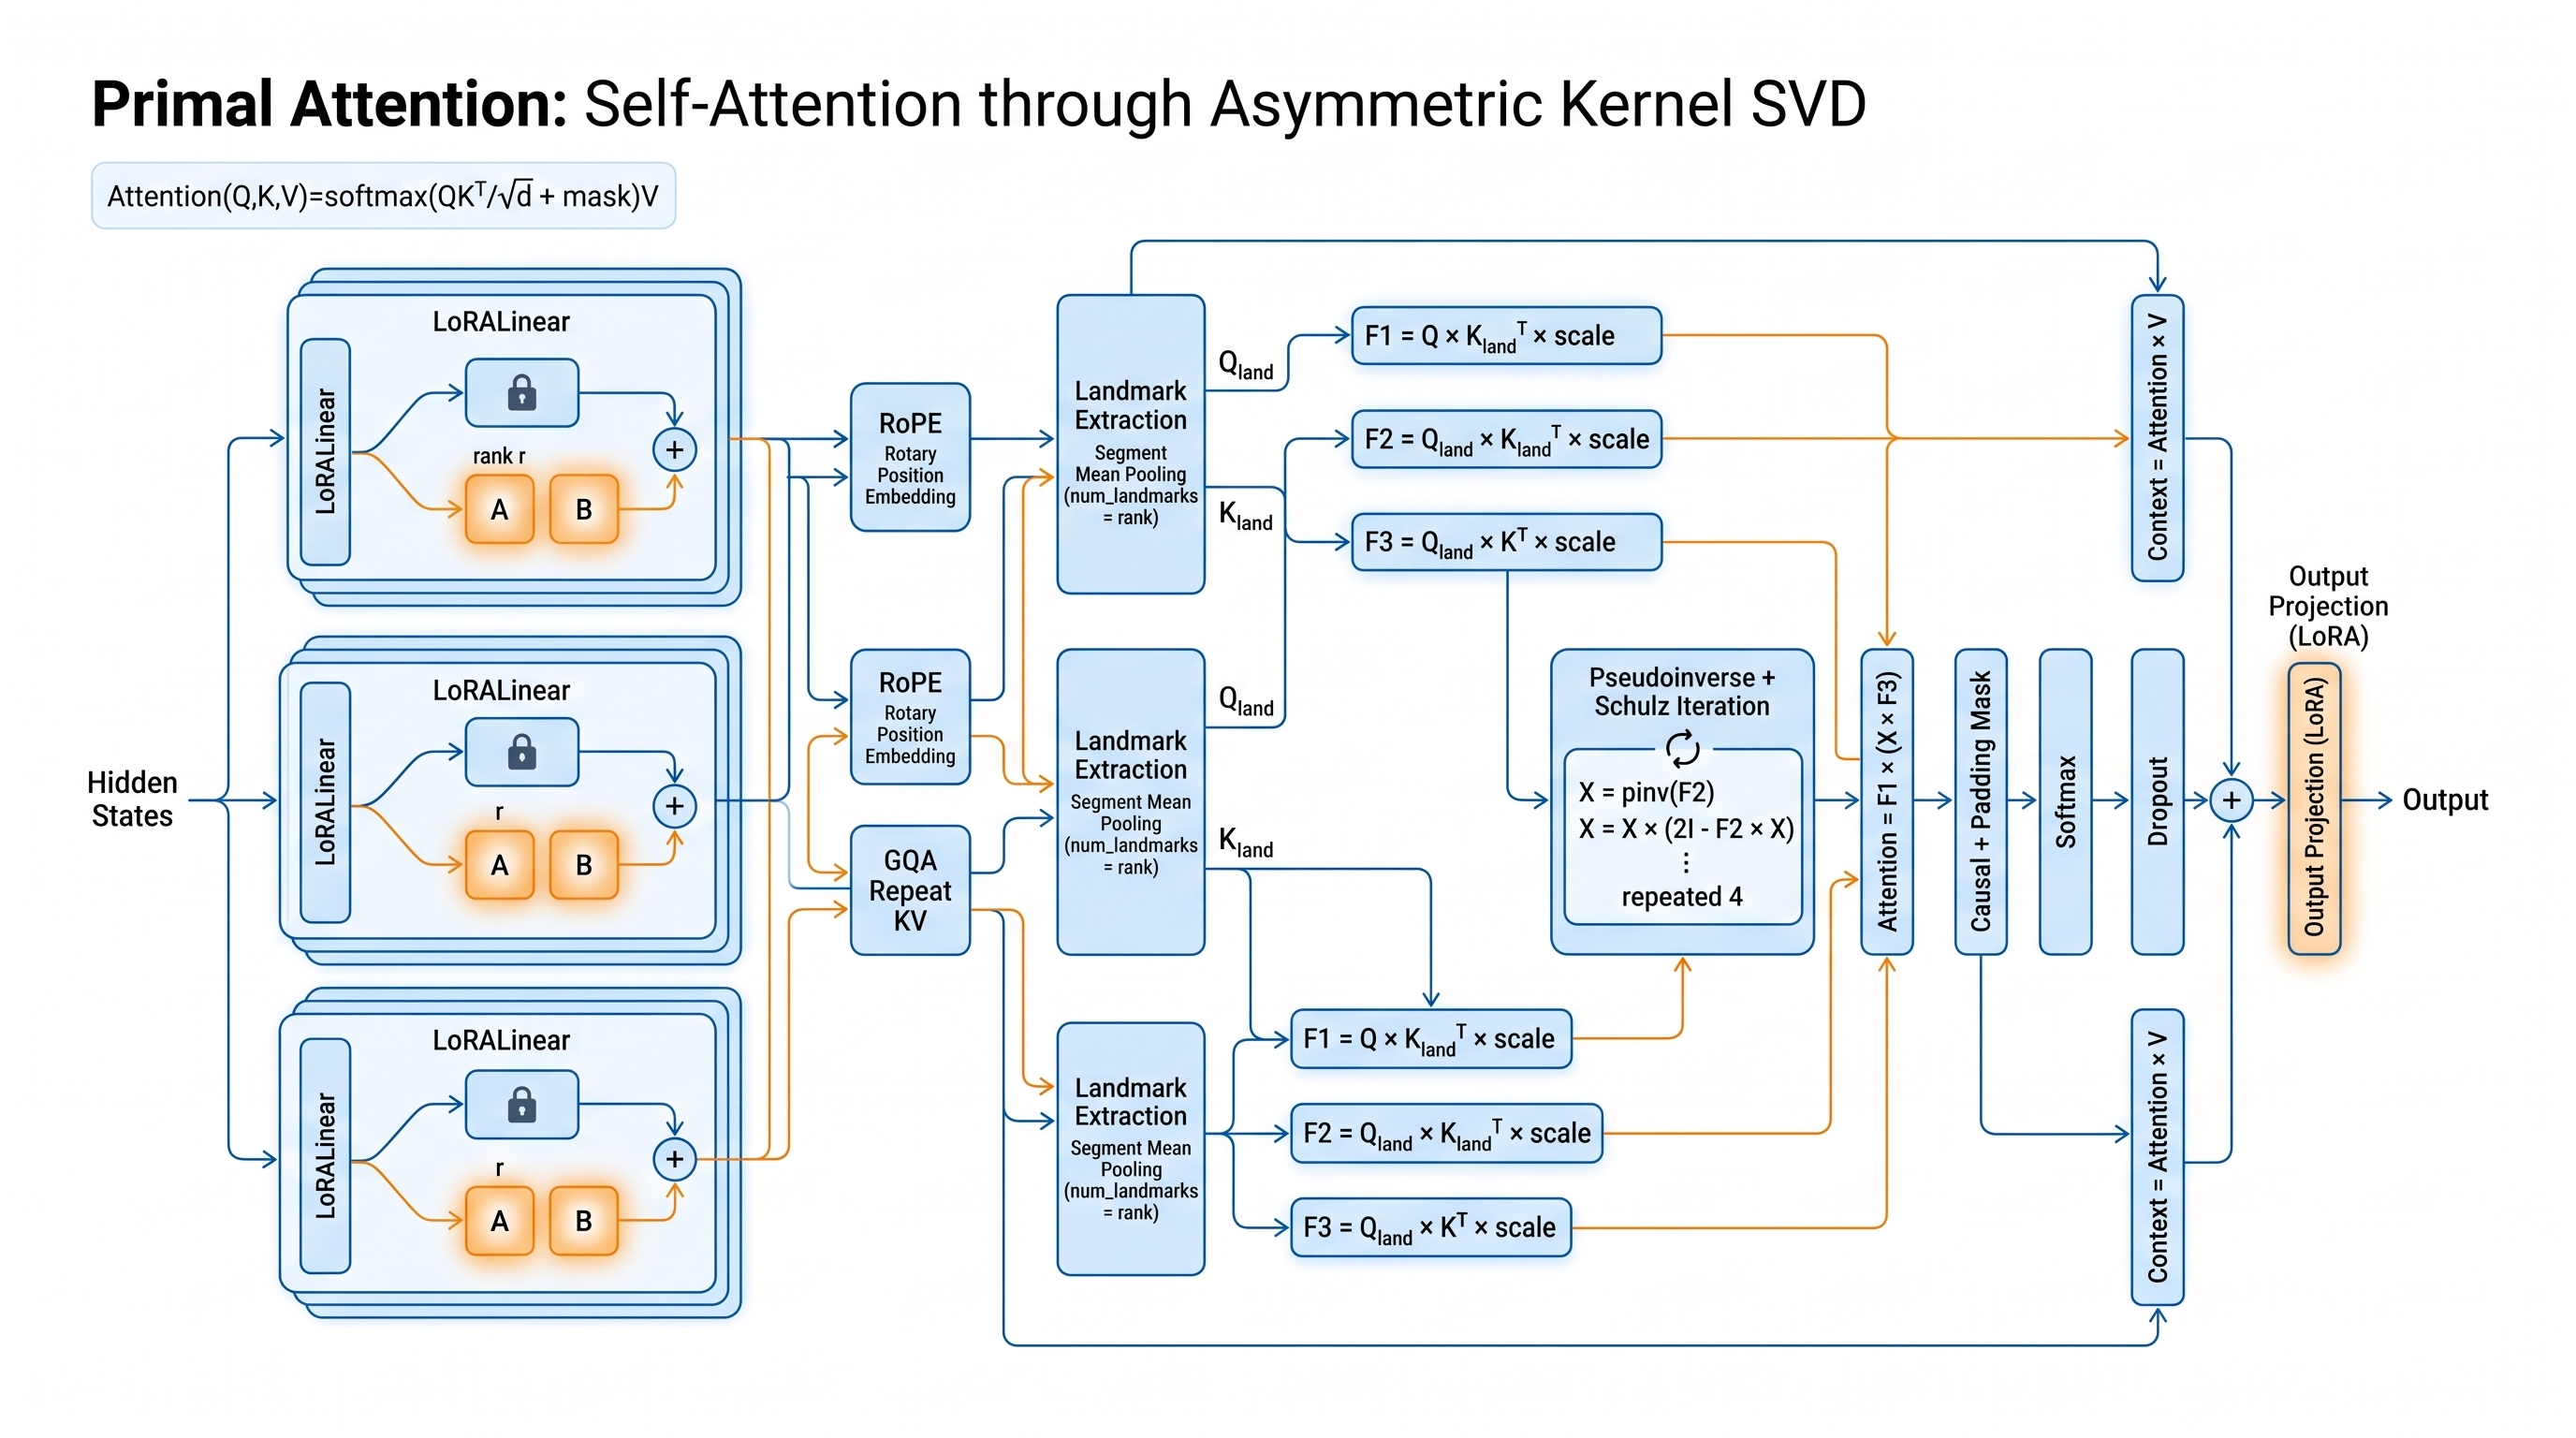
\includegraphics[width=0.92\textwidth]{img/arch_primal_attention.jpeg}
\caption{دیاگرام ساختار معماری و جریان تانسوری ماژول \lr{(primal\_attention)}}
\label{fig:arch_primal_attention}
\end{figure}

\begin{figure}[H]
\centering
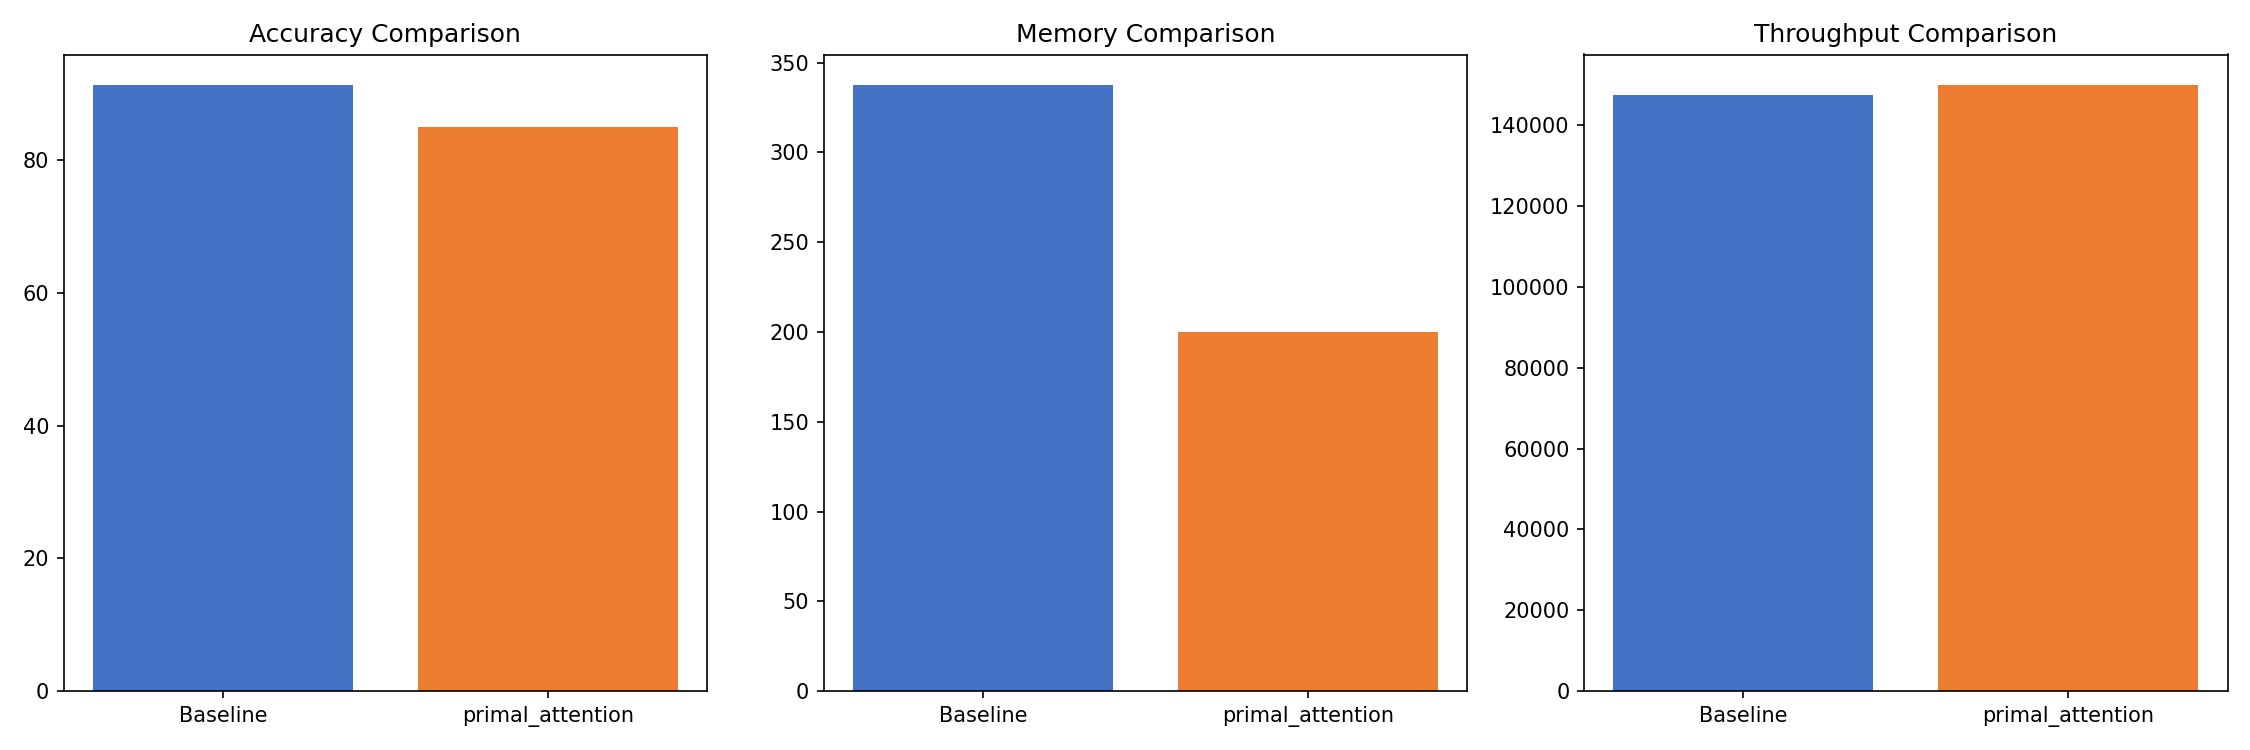
\includegraphics[width=0.92\textwidth]{img/comparison/primal_attention_comparison.png}
\caption{نمودار ارزیابی مقایسه‌ای سه‌شاخصی مکانیزم در برابر خط مبنا \lr{(primal\_attention)}}
\label{fig:comp_primal_attention}
\end{figure}
